\icode{N23-ME-MU-L3-261019-002}
\nceeID[6]{2023全国乙}{21}如图，一质量为\(M\)、长为\(l\)的木板静止在光滑水平桌面上，另一质量为\(m\)的小物块(可视为质点)从木板上的左端以速度\(v_0\)开始运动。已知物块与木板间的滑动摩擦力大小为\(f\)，当物块从木板右端离开时\paren[]
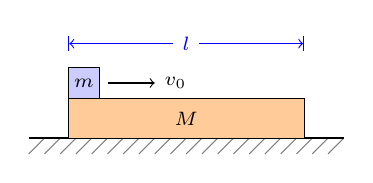
\begin{tikzpicture}[font=\scriptsize]
	\foreach \x in {0,.2,...,3.8}
		\draw[gray] (\x,-.2)--++(.2,.2);
	\draw[thick] (0,0)--(4,0);
	\draw[fill=orange!40] (.5,0) rectangle(3.5,.5)node[midway]{\(M\)};
    \draw[fill=blue!20] (.5,.5) rectangle(.9,.9)node[midway]{\(m\)};
	\draw[|<->|,blue] (.5,1.2)--node[fill=white]{\(l\)}(3.5,1.2);
	\draw[->] (1,.7)--(1.6,.7)node[right]{\(v_0\)};
\end{tikzpicture}
\begin{choices}
	\item 木板的动能一定等于\(fl\)
	\item 木板的动能一定小于\(fl\)
	\item 物块的动能一定大于\(\frac{1}{2}mv_0^2-fl\)
	\item 物块的动能一定小于\(\frac{1}{2}mv_0^2 -fl\)
\end{choices}
\begin{answer}
    
\end{answer}